% !Mode:: "TeX:UTF-8"
\RequirePackage[l2tabu, orthodox]{nag}

\documentclass[twocolumn]{article}
	\usepackage[UKenglish]{babel}
	\usepackage{ragged2e}
	\usepackage[parfill]{parskip}
	\usepackage[a4paper]{geometry}
	\usepackage[english]{isodate}
	\usepackage{fullpage}
	\usepackage{graphicx}
		\graphicspath{{../fig/}}
	\usepackage{siunitx}
		\sisetup{separate-uncertainty}
	\usepackage{url}
	\usepackage{microtype}
	\usepackage[colorlinks=false, pdfborder={0 0 0}, unicode=true]{hyperref}
	\usepackage[backend=bibtex,sorting=none,giveninits=true,maxnames=3,citestyle=numeric-comp]{biblatex}
%		\bibliographystyle{ieeetr}
%		\addbibresource{../bib/biblo} %Insert Bibliography file name
		\addbibresource{../bib/cust}
		\setlength\parindent{0pt}
	\usepackage{subcaption}
	\usepackage{float} 
	\usepackage{commath}
	\usepackage{amsfonts}
	\usepackage{booktabs}
		\setlength\heavyrulewidth{1.5pt}
		\renewcommand{\arraystretch}{1.2}
	\usepackage[titletoc, title]{appendix}
	\usepackage[capitalise]{cleveref}
		\crefname{appsec}{Appendix}{Appendices}
	\usepackage{rotating}

	\usepackage{titling}
	\usepackage{color}

%	\usepackage{titlesec}
%		\titleformat{\section}{\normalfont\huge\bfseries}{\thechapter.}{20pt}{\huge}

	\usepackage[compat=1.1.0]{tikz-feynman}
	
	\usepackage[raggedright]{titlesec}		% Formating of headers and titles
	\usepackage[normalem]{ulem}         % Formating of headers and titles
	
	\definecolor{mygreen}{rgb}{0.152, 0.7, 0.375}
	\definecolor{mygray}{rgb}{0.5,0.5,0.5}
	\definecolor{mymauve}{rgb}{0.555, 0.266, 0.676}
	\definecolor{myblue}{rgb}{0.16, 0.5, 0.722}	

\newcommand{\subtitle}[1]{%
	\posttitle{%
		\par\end{center}
	\begin{center}\Large#1\end{center}
	\vskip0.5em}%
}
\newcommand{\pkg}[1]{\textsc{#1}}
\newcommand{\pythia}{\pkg{Pythia}}
\newcommand{\delphes}{\pkg{Delphes}}
\newcommand{\around}{{\raise.17ex\hbox{$\scriptstyle\sim$}}}
\newcommand{\gev}{\giga\electronvolt}

% Section Headers
%\titleformat{name=\subsubsection,numberless}{\normalfont\normalsize}
%\titleformat{name=\subsection,numberless}{\bfseries\normalsize}
%\titleformat{name=\section,numberless}{\bfseries\Large\filcenter}{}{0em}{#1}
%Document information

\title{Machine Learning Based Simulation of Particle Physics Detectors}

%\subtitle{Part III Project Report}
%\author{Seyon \textsc{Sivarajah}, Churchill College, ss2165}
%\author{Candidate Number: \\
%Supervisor: Dr. Christopher \textsc{Lester}}

\date{\printdate{2017-05-15}}

%End Document information

\begin{document}
\begin{titlepage}
	
	\newcommand{\HRule}{\rule{\linewidth}{0.5mm}} % Defines a new command for the horizontal lines, change thickness here
	
	\center % Center everything on the page
	
	%----------------------------------------------------------------------------------------
	%	hEADING SECTIONS
	%----------------------------------------------------------------------------------------
	\includegraphics[scale=0.1]{cambridge.png}\\[1cm] % Include a department logo
	\textsc{\LARGE University of Cambridge}\\[1.5cm]
	\textsc{\Large Department of Physics}\\[0.5cm]
	\textsc{\large Part III Project Report}\\[0.5cm]
	
	%----------------------------------------------------------------------------------------
	%	tITLE SECTION
	%----------------------------------------------------------------------------------------
	
	\HRule \\[0.4cm]
	{ \huge \bfseries Machine Learning Based Simulation of Particle Physics Detectors}\\[0.4cm] % Title
	\HRule \\[1.5cm]
	
	%----------------------------------------------------------------------------------------
	%	aUTHOR SECTION
	%----------------------------------------------------------------------------------------
	
	\begin{minipage}{0.4\textwidth}
		\begin{flushleft} \large
			\emph{Candidate Number:}\\
			8286W
		\end{flushleft}
	\end{minipage}
	~
	\begin{minipage}{0.4\textwidth}
		\begin{flushright} \large
			\emph{Supervisor:} \\
			Dr. Christopher \textsc{Lester} % Supervisor's Name
		\end{flushright}
	\end{minipage}\\[2in]
	
	%----------------------------------------------------------------------------------------
	%	lOGO SECTION
	%----------------------------------------------------------------------------------------
	
	%\includegraphics[scale=0.4]{}\\[1cm] % Include a department logo
	
	%----------------------------------------------------------------------------------------
	
	%----------------------------------------------------------------------------------------
	%	dATE SECTION
	%----------------------------------------------------------------------------------------
	
	{\large \printdate{2017-05-15}}\\[2in] % Date, change the \today to a set date if you want to be precise
	
	

\vfill % Fill the rest of the page with whitespace
	
\end{titlepage}
%\begin{titlepage}
%\maketitle
%
%
%%\begin{center}
%%\begin{tabular}{lr}
%%
%%%Experiment Performed: &  \\
%%
%%Supervisor: & Dr Christopher Lester\\
%%
%%%Experiment Title: & 
%%\end{tabular}
%%\end{center}
%
%\end{titlepage}
%------------------ABSTRACT-------------------
\twocolumn[
\begin{@twocolumnfalse}
	
	\maketitle
	\pagenumbering{arabic}
	\begin{abstract}
	A key part of experimental particle physics is the simulation of a detector's response to an event. Current simulators are polarised between those that are fast and approximate and those that are accurate and slow. Generative Adversarial Networks (GANs) are a class of generative machine learning model which have demonstrated promise in producing artificial photo-realistic images. This study employs GANs for detector response simulation. Building on the work of Oliveira \textit{et al.}, data generated by the hadronisation system \pythia~and the detector simulator \delphes~are used to produce \textit{jet-images}, converting jet energy deposits in calorimeter cells to pixel intensities in a 2D image. A Locally Aware GAN (LAGAN) is trained to generate  counterfeits of two classes of such images: boosted $W$ from $W'$ decay, and QCD background. Generated images are seen to distinguish between the classes accurately, and match physical properties (transverse momentum, n-subjettiness) to a reasonable extent. Significant performance gains compared to current fast simulation is demonstrated. 
\end{abstract}

\tableofcontents
\vspace{0.5in}
\end{@twocolumnfalse}
]



\clearpage
%------------------Introduction-------------------
\section{Introduction}

\subsection{Motivation}
Particle physics experiments involve colliding particles and measuring the properties of the objects produced. However, a given event could not only result in a variety of particle showers, but the response of the detector is also stochastic in nature. It is from this determination of track properties and object momenta that a physicist must infer the original event. Detector simulations are widely used to help with the inference by calculating what a response and output for a given event would be, and as such can be used as predictive tools for models.

Full, accurate simulations (AS) of the progress of particles through detectors, such as the commonly used \pkg{Geant} 4 \cite{geant4}, can produce extremely accurate predictions of the measurements. However, they are computationally expensive. Approximate, fast simulators (FS), such as \pkg{Delphes} \cite{delphes}, perform cruder calculations with a significant speed gain (AS \around10-1000s/event and FS \around0.01-1s/event \cite{delphessl}). The accuracy-performance imbalance between these two solutions leaves room for other potential avenues. One such route is the use of Machine Learning (ML) tools.

Generative models in ML attempt to learn a given probability distribution via exposure to samples, and thus accurately generate new elements of that distribution. Their capability has recently been significantly boosted by the burgeoning fields of neural networks and associated deep learning. Once the learning process is complete, such networks are demonstrably fast for appropriate usage. As such, a generative model capable of learning to simulate detector responses may strike a better performance-accuracy balance than current FS. The ultimate goal of further work would be a generative model which approaches an AS in terms of accuracy, at significantly lower computational costs.

\subsection{Existing Research}

Machine Learning has long been familiar to High Energy Physics (HEP), due to it being a highly statistical field. Recently, however, ML and associated fields have received significant research attention in computer science, technology and engineering due to increases in computing power and demonstrations of the power and versatility of such techniques. We are now beginning to see efforts towards bringing these new tools to bear in HEP.

Generative Adversarial Networks (GANs) \cite{gan1} are a subset of generative models which have recently come to the forefront of active research. This method trains two neural networks simultaneously, a generative model $G$ and discriminative model $D$. As the names suggest, G generates ``fake" data which D attempts to distinguish from the ``real" training data. As each network is trained to improve at their task, they compete such that ultimately G produces new data which is indistinguishable in theory from the original distribution. GANs have shown strong performance in generating and manipulating photo-realistic images \cite{Radford2015,odena2016conditional,learnww,text2im,GoodfellowNips}.

Jets from boosted particles is an active research field \cite{BOOST}, and where many ML tools are used.  This project focusses on work done using jet-images produced by mapping jet energy deposits to an image \cite{cogan2014jet,de2015jet}, particularly boosted jet identification \cite{Komiske:2016rsd,Almeida:2015jua,Baldi:2016fql}. Earlier this year, GANs were trained on jet-images generated from \pkg{Pythia} output (hadronisation and parton showers \cite{pythia}) and showed promise in replicating physical distributions \cite{de2017learning}. This represents an initial foray in to using generative models for HEP. Recent work has also demonstrated classification of jets using ML techniques from natural language processing \cite{louppe2017qcd}.

\subsection{Report outline}

This report details an application of GAN based learning to jet-images from \pkg{Delphes} (FS) output, building on the work of Oliveira \textit{et al}. \cite{de2017learning} who demonstrated the principle for \pkg{Pythia} data. Jet-images were produced and pre-processed from \pkg{Delphes} output files, then used as training data for a GAN architecture. The trained network was then used to generate ``fake" images. The quality of this output was assessed by comparison to the training set. 

The following chapter outlines the theoretical background of GANs and the boosted jet process considered. \Cref{sec:methods} describes the methods employed, and \cref{sec:results} presents and discusses the outcomes of the training process. Final conclusions are presented in \cref{sec:conclusions}.
\vfill
%------------------Theory-------------------
\section{Background \& Theory}
\label{sec:theory}


\subsection{Detectors \& Simulations}
\label{sec:detector}

\begin{figure*}[!htbp]
	\centering
	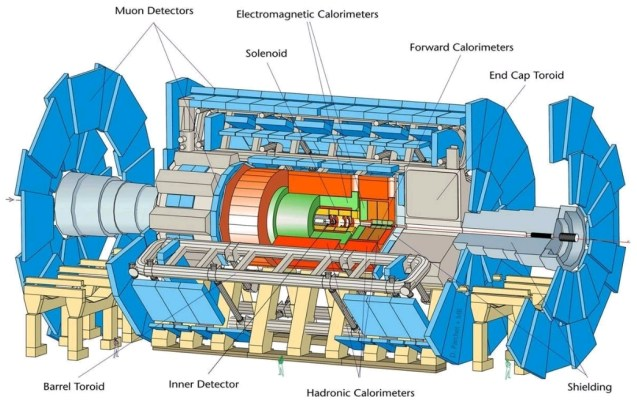
\includegraphics[width=0.8\textwidth]{atlasdetector}
	
	\caption{Cutaway diagram showing components of ATLAS detector. Source: \cite{atlaspic}}
	\label{fig:atlaspic}
	
\end{figure*}


Modern particle detectors are a complex set of measurement systems working in unison. Taking as an example the ATLAS experiment, we can see in \cref{fig:atlaspic} a cutaway of the detector set up. Simplistically, the energy and momentum of particles travelling out from the collision are measured by the calorimeters. The solenoids create a controlled magnetic field, the direction of travel in the field and the curvature of the particles gives a measurement of charge and mass respectively. A detailed description of the detector can be found in Ref. \cite{armstrong}.

The response of a detector to a particular particle event is therefore non-trivial to predict, particularly due to the high degree of stochastic variation between any two measurements. A significant difficulty faced by LHC experiments is the jets of hadronisation produced by quarks or gluons, as only the final branches of the jets are measured by the calorimeters. Without an understanding of this response, however, a physicist cannot infer the event that took place, or indeed make predictions about measurements that will be made. It is in this arena that simulations of detector behaviour are crucial. 

\cref{fig:simdiag} outlines a typical simulation sequence. The first step in the process is a matrix element calculator, which for this investigation is the commonly used MadGraph5 \cite{madgraph}. This piece of software loads a given model (particles and interactions), and calculates all the tree-level diagrams which take the given initial particles to the final particles. Using this information, Monte-Carlo methods are used to calculate the matrix element using a given number of events. Next, an event generator, \pkg{Pythia} in this case, calculates the subsequent interactions, decays parton showers and performs hadronisation \cite{Gieseke2012}.

The results of this are the``truth events", which for our purposes is the input, $\mathbf{x}$, to any simulator under consideration. The simulator performs two key tasks, that of calculating the response of the detector as the particles travel through it, and reconstructing the underlying events from such information. The reconstruction step is performed in much the same way as actual experiments, so is a useful representation of the simulated results.

An AS then propagates the input through a detailed model of the detectors to calculate the response. \pkg{Delphes}, the FS under consideration, takes a modular approach by separating the various components of the detector and performing approximate calculation and addition of stochasticity at each stage. Details of this can be found in \cite{delphes}, a summary is shown in \cref{fig:delphes}.        
\vfill
\begin{figure*}[!htbp]
	\centering
	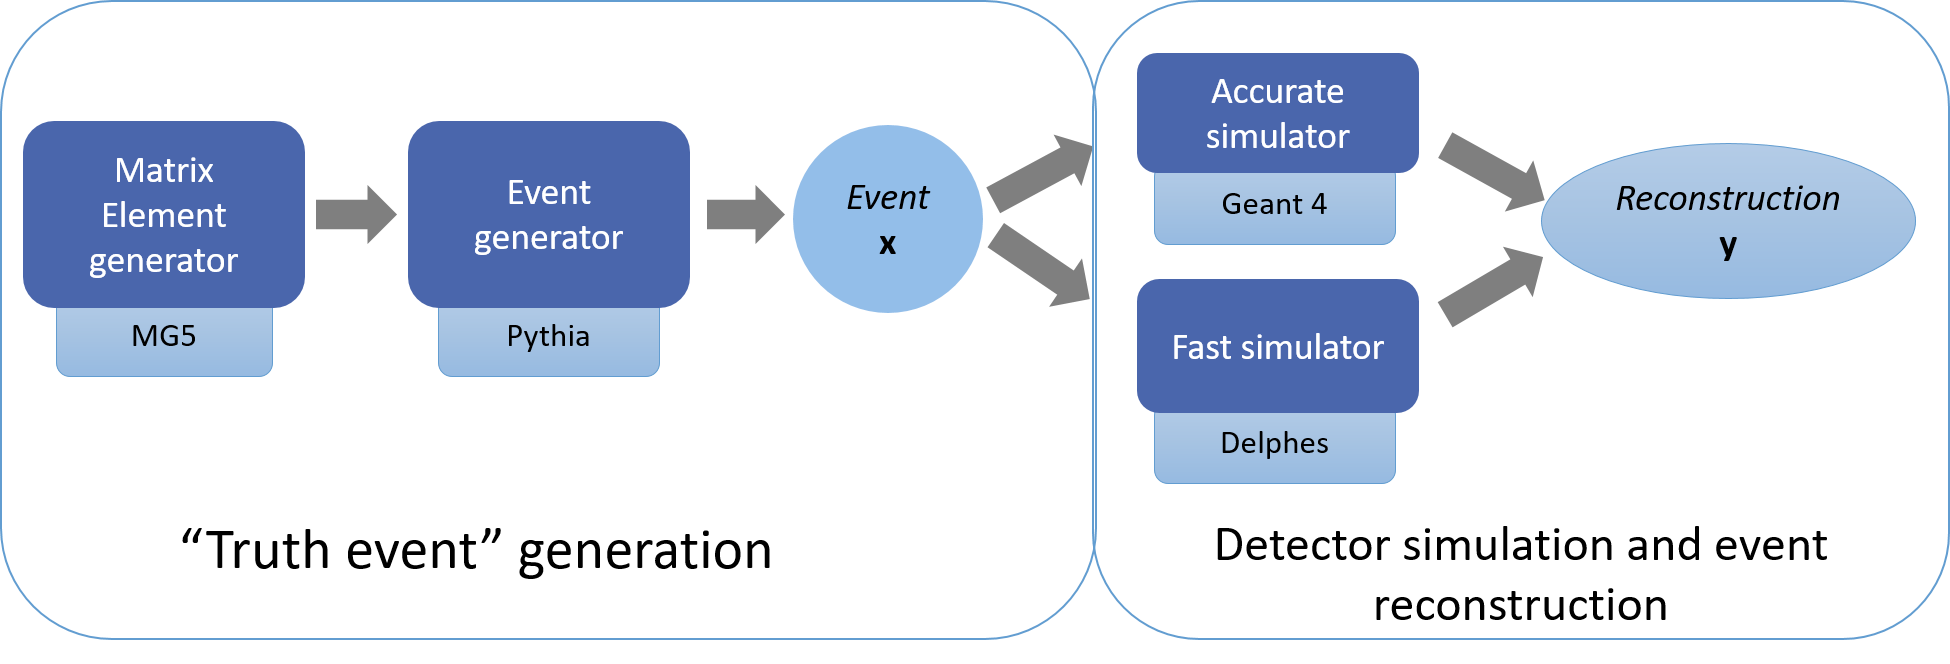
\includegraphics[width=0.8\textwidth]{simdiag}
	
	\caption{Summary of simulation process, from matrix element generation to final reconstruction from detector response.}
	\label{fig:simdiag}
	
\end{figure*}	

\begin{figure}[H]
	\centering
	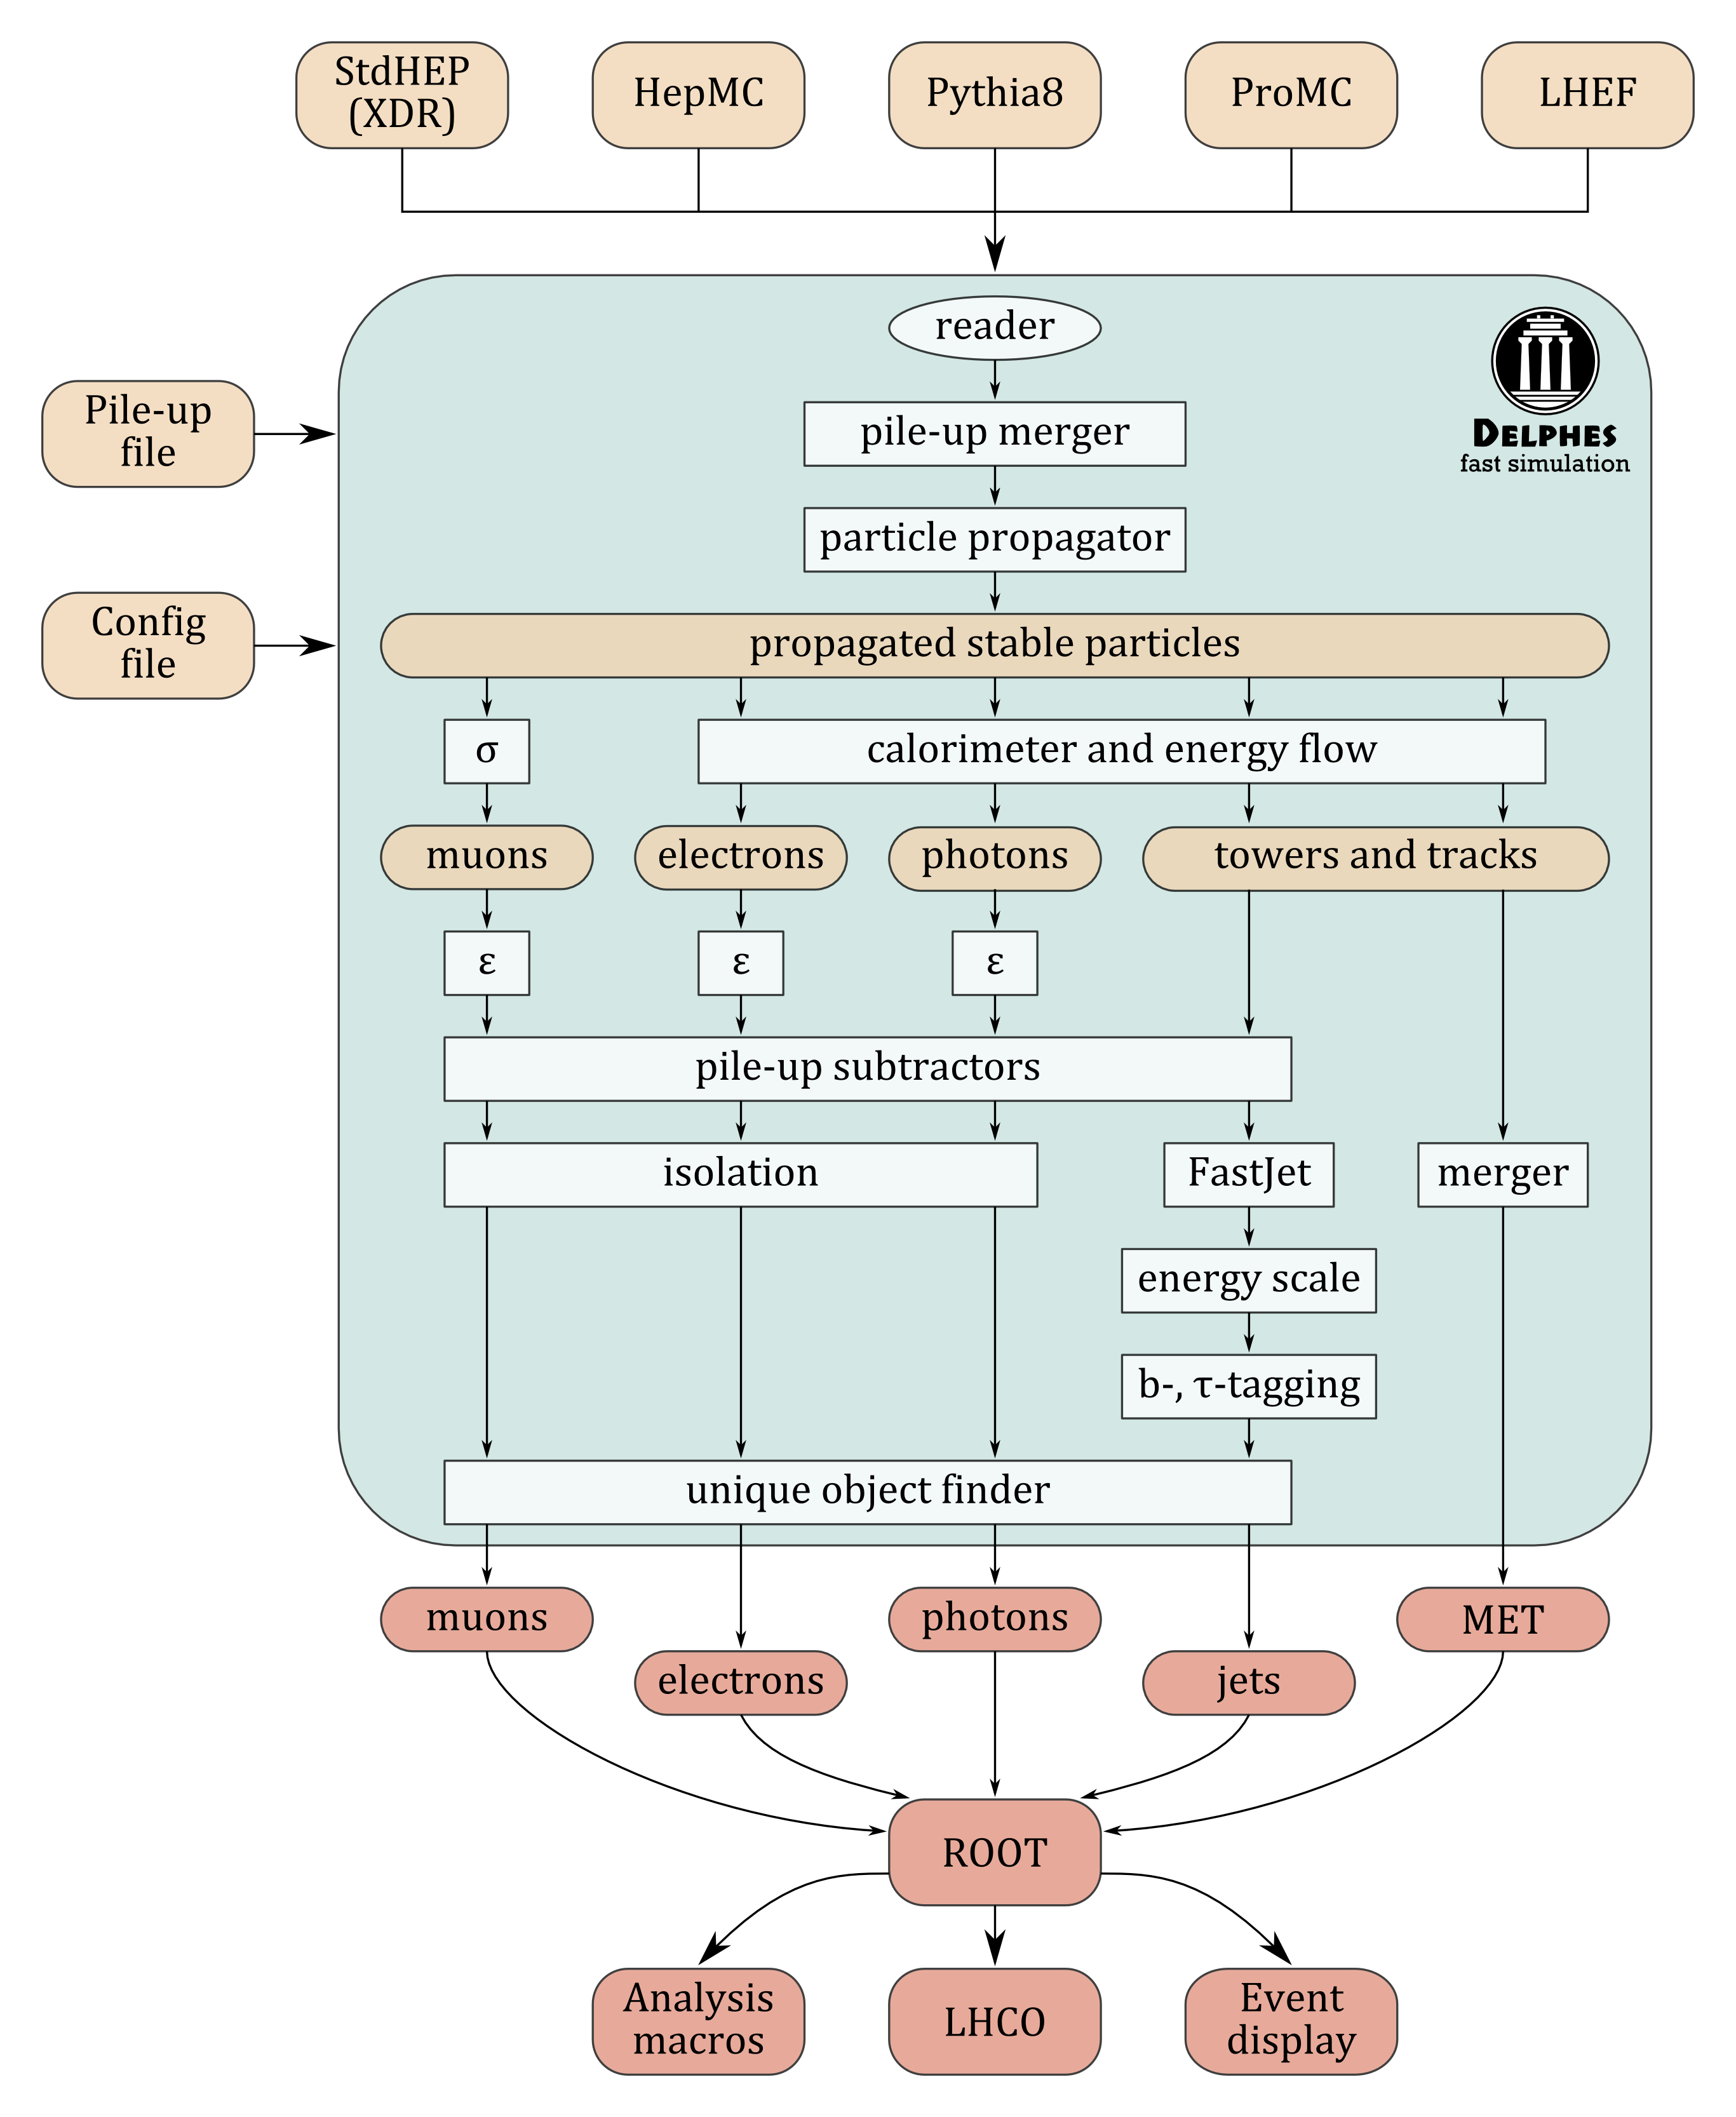
\includegraphics[width=1.0\columnwidth]{delphes}
	
	\caption{Summary of \pkg{Delphes} modules and function. Source: \cite{delphesslid}}
	\label{fig:delphes}
	
\end{figure}

 
\subsection[Generative Adversarial Networks]{\protect\raggedright Generative Adversarial Networks}
\label{sec:ml}

Traditional and well developed machine learning can be understood very much in parallel with the Bayesian methods of experimental physics. We attempt to determine the most likely parameters, $\theta$, for a given model, $\mathcal{M}$, for measurements $y$. This probability, $p(\theta|y, \mathcal{M})$, is the posterior. It is usually done by maximising the likelihood (probability of data given parameters) \cite{data}:

\[
p(y|\theta, \mathcal{M}) = \frac{p(\theta|y, \mathcal{M})p(y|\mathcal{M})}{p(\theta|\mathcal{M})}
\]

In machine learning, computers perform this task using training data to learn the parameters, then subsequently make predictions on new data. Typically these actions are classification (labelling), regression (common in physics) and clustering (similarity of data points). 

More recent developments have made significant inroads into \textit{generative} models, wherein learning is done in order to produce new samples of data. In particular neural networks and deep learning have played a large role, as neural networks scale well with dimensions, are end-to-end differentiable (crucial for gradient based training) and can represent complex functions \cite{deepgen}.

%here is where GAN lit review needs to go.

In the simplest case GANs consist of two competing networks $G$ and $D$. $G$ takes a latent noise variable $z$ as input and outputs artificial data $\mathbf{y} = G(z;\theta_g)$, where $\theta_g$ are the parameters of the network. $D$ takes either real or artificial data as input and outputs a scalar, $D(\mathbf{y})$, corresponding to the probability that $\mathbf{y}$ is real. $G$ is trained to improve at fooling $D$ and $D$ is trained to improve at distinguishing real data from generated. This can be described by a min-max game with value function $V(G,D)$:

\begin{equation}
	\label{eq:minmax}
	\begin{split}
	\min_{G}\max_{D}V(D,G) &= \mathbb{E}_{\mathbf{y}\sim p_{\text{data}}(\mathbf{y})} [\log(D(\mathbf{y})]\\
	&  +\mathbb{E}_{\mathbf{z}\sim p_{z}} [\log(1-D(G(z)))],
	\end{split}
\end{equation} 

where  $\mathbb{E}_{\mathbf{y}\sim p_{\text{data}}(\mathbf{y})}$ expresses expectation over the data probability distribution. The system is summarised in \cref{fig:gandiag}.

It can be shown that there exists a unique solution to this, a saddle point, strictly when $p_{\text{data}} = p_G$, where $p_G$ is the distribution produced by $G$ \cite{gan1}. This theoretical guarantee is a key advantage of GANs, as well as the ability to train them using standard back propagation algorithms and the lack of Markov Chains which are often needed in other generative models. By modifying the parameters to bring the system closer to this optimum (training, e.g. by a gradient descent method such as ADAM \cite{adam}), we achieve a successful data generation scheme.   

\begin{figure}[H]
	\centering
	\includegraphics[width=1.0\columnwidth]{goodgan}
	
	\caption{Generative Adversarial Nets process. Source: \cite{GoodfellowNips}}
	\label{fig:gandiag}
	
\end{figure}
 

\subsection{Boosted Jets}

The LHC has been able to probe unprecedented energy scales, especially with the upgrade to \SI{13}{\tera\electronvolt} operation. For the first time, large numbers of massive particles (i.e. $W$, $Z$, top quark, Higgs boson) are being produced with transverse momenta $p_T$ considerably larger than their rest mass $m$. Traditional reconstruction techniques identify all the decay products of such objects as a single jet, making distinguishing such jets from the large background of QCD jets a prominent problem \cite{BOOST}. As these \textit{boosted} objects may also include contributing effects from physics beyond the standard model, there is considerable active study in this area.

Modern methods probe individual jets and their detailed substructure for identification and tagging. A key property is the number of hard `prongs' of radiation in a jet. Electroweak boosted objects ($W/Z/H$) produce two prongs, while a boosted top quark produce three \cite{nsubjettiness}. Background QCD processes only lead to a single hard prong \cite{prongs}.

The process considered in this investigation is the decay of a $W'$ boson, which, along with $Z'$, are massive gauge bosons which arise in extensions to electroweak theory. The simplest example of which is imposing an extra $SU(2)$ symmetry, i.e. $SU(2)_1 \times SU(2)_2 \times U(1)$, which gets spontaneously broken resulting in the standard electroweak $SU(2)$ \cite{pdg2012}. These particles are predicted to have masses on the order of \si{\tera\electronvolt}. The decay sequence imposed in this project is given by the Feynman diagrams in \cref{fig:feynmans}.


	\begin{figure}[]
		\centering
		\begin{subfigure}[t]{1.0\columnwidth}
			\centering
			\feynmandiagram [horizontal=a to b] {
				i1 [particle=\(f\)] -- [fermion] a -- [fermion] i2 [particle=\(\bar{f}\)],
				a -- [photon, edge label=\($W'$\)] b,
				f1 [particle=\(W\)] -- [photon] b -- [photon] f2 [particle=\(Z\)],
			};
		\end{subfigure}%
		\\ 
		\begin{subfigure}[t]{0.45\columnwidth}
			\centering
			\feynmandiagram [horizontal=a to t1, small] {
				a [particle=\(W\)] -- [photon] t1,
				p2 [particle=\(q'\)] -- [fermion] t1 -- [fermion] p1 [particle=\(q\)],
			};
		\end{subfigure}
		~
		\begin{subfigure}[t]{0.45\columnwidth}
			\centering
			\feynmandiagram [horizontal=a to t1, small] {
				a [particle=\(Z\)] -- [photon] t1,
				p2 [particle=\(\bar{\nu}\)] -- [fermion] t1 -- [fermion] p1 [particle=\(\nu\)],
			};
		\end{subfigure}
	\caption{Feynman diagram for process under consideration. Fermion annihilation produces $W'$ decaying to boosted $W$ and $Z$.}
	\label{fig:feynmans}
	\end{figure}

The large mass of the decaying $W'$ means the $W$ is highly boosted, and decays to quarks producing a boosted jet. By forcing the $Z$  boson to decay to neutrinos, we ensure it does not complicate our signal; it decays ``silently". The boosted $W$ is expected to produce a two-pronged pattern. This study contrasts this process with background QCD jets.
 


%------------------Method-------------------



\section{Methods}
\label{sec:methods}

\subsection{Jet-images}
\subsubsection{Calorimeter to image}
The jet-image generation largely follows the scheme described in Ref. \cite{de2015jet}, adapted for extraction from \pkg{Delphes} output \pkg{ROOT} files. Training data generation begins by running \pkg{Delphes}3 (with internal \pkg{Pythia}) using the \textit{DelphesPythia8} command \cite{workbook}. \pkg{Pythia} is configured for collisions at $\sqrt{s} =$ \SI{13}{\tera\electronvolt}, and a $W'$ boson mass of \SI{800}{\giga\electronvolt}. \pkg{Delphes} is configured to use the \pkg{FastJet} \cite{fastjet} package for jet-clustering (assigning particles to jets) using the anti-$k_t$ algorithm \cite{antikt}, with a radius parameter of $R=1.0$. The jet in each event with the highest transverse momentum is selected for the image. Trimming is also performed in this step, see \cref{sec:preproc} for details.

The output \pkg{ROOT} file (see \cref{fig:delphes}) is processed to extract information about jet constituents. Jet-image axes correspond to the orthogonal directions of azimuthal angle $\phi$ and pseudorapidity $\eta$; pseudorapidity is defined by the azimuthal angle $\theta$ as $\eta \equiv -\ln(\tan(\theta/2))$. Pixels of size $0.1 \times 0.1$ span a grid of angle values $\eta \times \phi \in [-1.25, 1.25]\times [-1.25, 1.25]$, forming a $25\times 25$ pixel image. The intensity of pixel $i$, denoted $I_i$, is given by the sum of transverse energies (assuming clusters are massless, as shown in \cref{app:pixels}) over all the calorimeter cells that fall within the pixel\footnote{The longitudinal segmentation of calorimeter towers is collapsed to a flat cylinder in our idealised picture}, indexed by c, 

\begin{equation}
I_i = \sum_c p_{T, i}^{(c)} = \sum_c\frac{E^{(c)}_i}{\cosh{\eta^{(c)}}_i} ,
\label{eq:intensity}
\end{equation}

where $E^{(c)}$ and $\eta^{(c)}$ are the energy and pseudorapidity of cell $c$. \Cref{fig:calangle} shows a particle hitting an idealised cylindrical calorimeter tower configuration with a superimposed pixel grid.

%\begin{figure}[]
%	\centering
%	\includegraphics[width=0.5\linewidth]{etaphi}
%	
%	\caption{Relationship between spherical polar angles and pseudorapidity. Source: \cite{etadiag}}
%	\label{fig:etadiag}
%	
%\end{figure}

\begin{figure}[H]
	\centering
	\includegraphics[width=1.0\columnwidth]{calangle}
	
	\caption{Idealised cylindrical calorimeter tower arrangement, with particles colliding along the $z$ axis. A scattered particle hits a calorimeter cell within pixel $i$ at polar angle and pseudorapidity values $\phi$ and $\eta$. Pixel division sizes are not representative; pseudorapidity diverges when approaching the $\pm z$ axis.}
	\label{fig:calangle}
	
\end{figure}

\subsubsection{Pre-processing}
\label{sec:preproc}

Pre-processing the images to exploit the inherent physical symmetries and remove obfuscating variations significantly improves performance. The steps employed are as follows:

\begin{enumerate}
	\item \textbf{Trimming} \cite{trimming}: The anti-$k_t$ algorithm is applied to the jet to cluster it in to sub-jets with $R = 0.3 k_t$, and those with less than 5\% of the transverse momentum of the overall jet are dropped. This helps to highlight the hard event under consideration, and reduces the effect of pileup (multiple proton-proton collisions in the same event). The trimming step is carried out in the initial \pkg{Delphes} run, via \pkg{FastJet}.
	
	
	\item \textbf{Translation}: Using the sub-jet information from the trimming step, the jet is translated so that the sub-jet with highest transverse momentum is at the centre of the image. This step is performed when initially pixelising the calorimeter measurements. Translations in $\phi$ are rotations about the collision axis, so pixel intensities are invariant. However, translations in $\eta$ are Lorentz boosts. With the pixel intensity as defined in \cref{eq:intensity}, the pixel intensity also remains invariant under such translations (see \cref{app:pixels}).

	\item \textbf{Rotation}: Once the image has been read in, it is rotated such that the sub-leading jet is directly below the leading, i.e. at an angle of $-\pi/2$ with the origin at the centre of the image. If the angle of rotation is not a multiple of $\pi/2$, which in general it is not, the rotated pixel grid will not align with the original. Thus for a general affine rotation pixel intensity redistribution via interpolation is required, this is performed using a cubic spline interpolation. If no second sub-jet is present, the image is rotated such that the principle component axis is vertically downwards. To counter the effects of interpolation, the sum of intensities is renormalised to be equal to the value before rotation in order to minimise the information lost.
	
	\item \textbf{Flip}:  The image is reflected about the central vertical axis if required such that the right is always the half with the higher total intensity. This further helps make sure the hardest features (the ones of physical interest) appear in similar positions, aiding the training procedure. 
	
\end{enumerate}

The final three steps are demonstrated in \cref{fig:preproc} using a simplified image. \Cref{fig:ex_sig_real} shows a random sample image generated from \pkg{Pythia} + \pkg{Delphes} (PD) with all pre-processing steps applied, more samples are given in \cref{app:samples}. In order to marginalise the effect of variations in transverse momentum for this study, $p_T$ of jets used for training is restricted to \SI{250}{\giga\electronvolt} $\leq p_T \leq$ \SI{300}{\giga\electronvolt}. Similarly, a further cut on jet mass is imposed by requiring \SI{60}{\giga\electronvolt} $\leq m \leq$ \SI{100}{\giga\electronvolt}. Both cuts are performed using the value provided by the clustering algorithm for each jet.

All jet-image generation is performed using Python v2.7, using \pkg{PyROOT} (the Python interaction module for \pkg{ROOT} \cite{root}) to read in \pkg{Delphes} objects. \pkg{Numpy} \cite{numpy} is used for image processing, alongside \pkg{Scikit-image} \cite{skimage} for the rotation. \pkg{Matplotlib} \cite{matplotlib} was used to produce all plots in this report.

\begin{figure*}[!htbp]
	\centering
	\includegraphics[width=1.0\linewidth]{preproc_2}
%	\input{../fig/preproc_2.pdf_tex}
	
	\caption{Demonstration of final three pre-processing steps applied to jet-images produced from PD output, with a simplified toy image. Details of the steps are in the text.}
	\label{fig:preproc}
	
\end{figure*}

\begin{figure}[H]
	\centering
	\includegraphics[width=1.0\columnwidth]{ex_sig_real}
	
	\caption{Sample jet-image from \pkg{Pythia} + \pkg{Delphes} data after pre-processing. High intensity centre (leading sub-jet) and sub-leading sub-jet directly beneath are seen. Pixel values are plotted on a log scale. More samples are given in \cref{app:samples}.}
	\label{fig:ex_sig_real}
	
\end{figure}

\subsection{GAN}
The GAN architecture and training used are fully discussed in Ref. \cite{de2017learning}, and are summarised in this section.
 
\subsubsection{Architecture}
The Locally Aware GAN (LAGAN) architecture used builds upon the Deep Convolutional formulation \cite{Radford2015}, which essentially consists of several convolutional filter layers before the fully connected neural network. This helps identify and generate specific features in an image. Whereas in the convolutional case a filter patch is slid across the entire image, in the Locally Aware case patches are assigned to a given part of the image. Therefore rather than $N$ filters being convolved with the whole image, there are $N$ distinct filters applied per patch of image, which are trained independently. This is key to breaking translational invariance and producing well defined local features as required.

Further deviations from traditional GANs are required to compensate for differences between natural images and jet-images. Jet-image pixel intensities are not confined to a fixed range (such as 0 - 255 in an 8-bit grayscale image), but rather need to cover several orders of magnitude. Furthermore, in a given jet-image the majority of pixels have a null value leading to sparsity. The final non-linear activation layer in G is chosen to be a Rectified Linear Unit (ReLU) \cite{relu}, which performs the operation
$$
f(x) = \max(0, x)
$$
% APP NN
on an input $x$. This helps produce a large number of null cells, and unbounded maximum. 

A common disadvantage of GANs is a proclivity for G to overwhelmingly produce a single sample which D struggles to classify, this is known as \textit{mode-collapse} \cite{gan1}. Minibatch discrimination \cite{improvedgan}, used here, allows D to exploit batch-level features, making collapse unfavourable for G. It also proved key for achieving high dynamic range and sparsity.

An auxiliary classification task for the discriminator, as described in the ACGAN system \cite{odena2016conditional} is also employed. The Discriminator, as well as determining whether an image is real or fake, also assigns it a label corresponding to whether it is a `signal' ($W'$ jet) or `noise' (QCD jet). Similarly, the Generator is tasked with producing an image conditioned on an input label corresponding to the process. Both models are thus minimising a second loss function $L_C$ which can be expressed in terms of log-likelihoods as

\begin{equation}
\label{eq:acloss}
\begin{split}
L_C = &-\mathbb{E} [\log P(C=c~| X_{real})]\\ &- \mathbb{E} [\log P(C=c~| X_{fake})]
,
\end{split}
\end{equation} 
where $P(C=c~| X_{real})$ indicates the probability of the assigned class being correct given the sample $X$ is real.
This has not only been shown to aid the training process, but also demonstrates that a GAN could simulate a variety of physical processes, by conditioning on the input \cite{mirza2014conditional}.

\Cref{fig:stitch} shows the total architecture used in this LAGAN system. 
\begin{figure*}[!htbp]
	\centering
	\includegraphics[width=1.0\textwidth]{stitch}
	
	\caption{LAGAN architecture used for training. Source: \cite{de2017learning}}
	\label{fig:stitch}
	
\end{figure*}   

\subsubsection{Training}
\label{sec:training}
Training was performed with gradient descent using the ADAM optimiser \cite{adam}. The noise variable input to the discriminator was a normally distributed vector of length 200, with 0 mean and a standard deviation of 1. Training was performed on batches of 100 images at a time, for 50 epochs (total runs of training over the whole dataset). Models were built and trained using \pkg{Keras} v1.2 \cite{keras} with a \pkg{Tensorflow} v0.11 \cite{tensorflow} backend.

Training was performed for two training image datasets of size \around6k and \around25k, each set containing approximately equal numbers of the two classes of jet-image ($W'$ and QCD). A single training sequence on the larger dataset took approximately \SI{35}{\hour} to run on the computational resources available (CPU), and so was determined to be a reasonable maximum size. The original \pkg{Pythia} only investigation was able to use GPUs, which significantly reduce training time, thus the authors could make use of a 800k image dataset.


%---------------------------------RESULTS-----------------------------%
\section{Results and Discussion}
\label{sec:results}

This chapter presents and examines the outcomes of the investigation. \Cref{sec:delphes-ims} evaluates the effect of \delphes~on the produced training dataset of jet-images. The GAN generated images are presented in \cref{sec:genims}, and distributions they produce in associated jet variables are considered in \cref{sec:physical}. \Cref{sec:comp} briefly outlines the computational advantage of the scheme presented.

\subsection{Delphes jet-images}
\label{sec:delphes-ims}

As jet-images have not previously been produced from \delphes~output, we first characterise them. Superficially, as the general FS function is smearing of particle tracks and measurements, we would expect hard centres of radiation to be broadened and spread over the images from \pythia+\delphes~(PD) output, compared to purely \pythia~(P). Average images\footnote{Average images correspond to an array of the average value of each pixel over the set.} generated from \around\num{12500} images for both $W'$ (signal) and QCD (noise) decays are compared for P (data from the original investigation \cite{de2017learning}) and PD. 

\Cref{fig:delphes_ims} shows the sets of average images on a log scale for pixel intensity. A plot of difference between the images on a pixel by pixel basis (P - PD) is also shown, on a linear scale. The P images show circular symmetry in the low intensity regions away from the centre. The expected two hard prongs are seen in the $W'$ average, while the QCD prongs are broader, with the lower lobe at a smaller intensity. The PD images do not display the circular symmetry, likely because the low intensity region (\SI{e-4}{\giga\electronvolt} and below) is not captured by the dimensions of the image; it has been smeared out of frame. Further investigations should increase the dimensions to investigate this area.

As expected, the lobes of high intensity have been smeared in the PD images. The image of differences shows that in both cases the central, primary lobe, has a lower core intensity as compared to the P images, and it is spread mainly downwards in the $-\eta$ direction by \delphes. We may infer then that the smearing of the leading sub-jet is largely towards the sub-leading. The secondary lobe (which is not distinguishable in the QCD difference) is spread in to something akin to an arrowhead pointing downwards, though it is not well distinguished from the primary lobe in some areas. This suggests that again the smearing is biased towards the primary lobe, but now with a large tangential component. This effect may also be caused by lower efficacy of the jet-finding algorithm after detector response has been factored in. Thus the sub-jets may not be as accurately translated/rotated over all images.

The blurring of high intensity cores can be better understood by comparing the pixel intensities along the central vertical axis of the image, i.e.~$\eta=0$. This is shown in \cref{fig:delphes_middle}. The linear scale helps focus on the peaks. Central peaks broaden in the $-\eta$ direction, raising the intensity of the inter-lobe region significantly in both cases. While the distinctive $W'$ secondary peak broadens but remains visible, the previously small QCD secondary peak is now no longer separable from the decaying tail of the primary. Strict numerical conclusions are difficult to draw from so few points (low resolution image).


  
\begin{figure*}[!htbp]
	\centering
	\begin{subfigure}[t]{1.0\textwidth}
		\centering
		\includegraphics[width=1\textwidth]{av_PvPD_sig}
		\caption{$W'$ signal}
	\end{subfigure}%
	\\
	\begin{subfigure}[t]{1.0\textwidth}
		\centering
		\includegraphics[width=1\textwidth]{av_PvPD_noise}
		\caption{QCD noise}
	\end{subfigure}

	\caption{Comparison of average jet-images between those generated from just \pkg{Pythia} (P, left) and those also generated with \pkg{Delphes} (PD, right) on a log scale. The difference between the two images (P - PD on a pixel by pixel basis) is shown in the middle on a linear scale, with the colour map clipped to $\pm$\SI{20}{\giga\electronvolt} to aid visibility. Images for the $W'$ signal (top) and QCD noise (bottom) are shown. \pkg{Pythia} only images from Ref. \cite{de2017learning}. }
	\label{fig:delphes_ims}
\end{figure*}

\begin{figure*}[!htbp]
	\centering
	\includegraphics[width=1.0\textwidth]{av_PvPD_center}
	
	\caption{Pixel values for $\eta=0$ axis from average jet-images (over 12.5k images)  for $W'$ signal (left) and QCD noise (right), i.e. the average values of the signal axis.}
	\label{fig:delphes_middle}
	
\end{figure*} 

\subsection{Generated Images}
\label{sec:genims}

%Training as described in \cref{sec:training} was performed for two training datasets of size \around6k and \around25k, each set containing approximately equal numbers of each class of jet-image. This section first examines the results of the latter, the more fully trained. A single training sequence on this dataset took approximately 35 hours to run on the computational resources available, and so was determined to be a reasonable maximum size. 
This section first examines the results of the training performed on the larger 25k dataset, i.e. the more fully trained Generator (G). \Cref{fig:ex_sig_gen} is a random $W'$ sample from G (c.f. \cref{fig:ex_sig_real}), more samples are given in \cref{app:samples}. The generated images display the two key expected properties of sparsity (majority of the pixels are not activated), and the two high intensity regions at the centre and directly below the centre.

\begin{figure}[H]
	\centering
	\includegraphics[width=1.0\columnwidth]{ex_sig_gen}
	
	\caption{Sample jet-image produced by a LAGAN Generator after being trained on a 25k PD image dataset. Pixel values are plotted on a log scale. More samples are given in \cref{app:samples}}
	\label{fig:ex_sig_gen}
	
\end{figure}

\subsubsection{Average image comparison}
In order to assess the quality of the generated image distribution, a sample set was produced of the same size as the training PD set (12.5k images for each class). Average images are compared to the training data in \cref{fig:pdvg}, in the same fashion as \cref{fig:delphes_ims}. In the central and mid-range regions of the image the magnitude of intensities match training data, with a high intensity central region. Moreover, the $W'$ high intensity lobe also includes the secondary lobe, while the QCD lobe does not.

However, deficiencies in G images are readily apparent. The most clear is the empty outer regions of the averages, where negligible numbers of images have non-zero pixel values. This is largely due to the difficulties in achieving such large range in the output of the Generator. Training to achieve accuracy in the high intensity region comes at the price of a crude low intensity region. In the training data such pixels have intensities below \SI{e-2}{\gev}, four orders of magnitude below the centre. The ReLU activation layer, if insufficiently or incorrectly trained could have lead to too many pixels which are never activated.

Examining the difference images shows training images have higher intensity cores, but the generated images match to within 20\%. Notably, the G average image contains certain high intensity pixels in low intensity regions (especially for $W'$). Similarly, there are also certain pixels in high intensity regions which are never activated. This can be explained by some degree of mode-collapse, wherein G is disproportionately activating some pixels and never activating others. This can likely be overcome to an extent with a larger training set, the effect of dataset size is discussed more in \cref{sec:physical}.  

\begin{figure*}[!htbp]
	\centering
	\begin{subfigure}[t]{1.0\textwidth}
		\centering
		\includegraphics[width=1\textwidth]{av_GvPD_sig}
		\caption{$W'$ signal}
	\end{subfigure}%
	\\
	\begin{subfigure}[t]{1.0\textwidth}
		\centering
		\includegraphics[width=1\textwidth]{av_GvPD_noise}
		\caption{QCD noise}
	\end{subfigure}
	
	\caption{Comparison of average jet-images (over \num{12500} images) between training data (PD, left) and those from the trained Generator (G), on a log scale. The difference between the two images (PD - G) is shown in the middle on a linear scale. Images for the $W'$ signal (top) and QCD noise (bottom) are shown.}
	\label{fig:pdvg}
\end{figure*}


\subsubsection{Interim training images}
Some insight in to the training procedure and evaluation of the hyper parameters can be achieved by looking at intermediate results. For standard machine learning applications we could track training quality using the loss function. The GAN loss function (\cref{eq:minmax}), however, is notoriously not a useful measure of training, an issue recent reformulations are attempting to resolve \cite{wasserstein}.

We may instead examine the loss function for the auxiliary classification task (\cref{eq:acloss}). \Cref{fig:auxloss} shows the loss varying over the epochs of training (for the 25k dataset), evaluated on training sets of images and a separate test set, for both G and D (the equivalent plot for GAN loss is included in \cref{app:loss} for completeness). Also shown are average images from G at intermediate epochs for both classes. The loss variation suggests gains made beyond 20 epochs are marginal. This is somewhat supported by the images, which superficially vary little from this point onwards. The key difference between the two classes, two lobes for signal and one for noise, is seen to develop at around epoch 30. 

The value in further training may be seen in the sparsity. After beginning as random noise, initial learning produces a highly sparse average image with compact central cores. Subsequent images show more and pixels in the low-intensity regions being activated. While training up to or beyond 50 epochs may be useful in this regard, it is clear that more training data would be far more potent.

	\begin{figure*}[!htbp]
		\centering
		\includegraphics[width=0.8\textwidth]{auxloss}
		
		\caption{Variation in loss function for auxiliary task with training epoch, evaluated on training and testing data sets for Generator (G) and Discriminator (D) ((a), top). Average images from G at intermediate epochs for $W'$ signal and QCD noise ((b), bottom). The scale for pixel intensities is the same as previous figures, for example \cref{fig:pdvg}.} 
		\label{fig:auxloss}
		
	\end{figure*} 

\subsection{Physical Distributions}
\label{sec:physical}
Characterising a distribution of images, a 625 dimension distribution in the case of $25\times25$ pixels, is difficult to achieve numerically. Mapping images to a single variable, ideally a physically motivated one, gives a one dimensional distribution which could provide insight. Here we calculate two such distributions, the first is the `discretised' transverse momentum $p_T$ \cite{de2017learning}, calculated from the pixel values $I_i$ of an image $I$ as 

$$
p_T^2(I) = \bigg(\sum_i I_i \cos(\phi_i)\bigg)^2 + \bigg(\sum_i I_i \sin(\phi_i)\bigg)^2
$$

where $\eta_i$ and $\phi_i$ are the pseudorapidity and azimuthal angle, respectively. The second is n-\textit{-subjettiness} $\tau_{n}$ \cite{nsubjettiness}, which is a numerical measure of the extent to which a jet can be regarded as being composed of $n$ sub-jets (more likely to be $n$ sub-jets for smaller $\tau_n$). We can calculate the ratio $\tau_{21}$ using

$$
\tau_n (I) \propto \sum_i I_i \min_a \bigg(\sqrt{(\eta_i - \eta_a)^2 + (\phi_i - \phi_a)^2}\bigg),
$$

$$
\tau_{21} (I) = \tau_2 (I) / \tau_1 (I)
$$

where $\eta_a$ and $\phi_a$ are axis values determined with the one-pass kt axis selection using the winner-take-all combination scheme \cite{axis}. The ratio $\tau_{21}$ when measured for traditional jet data proves to be a useful distribution for discriminating two-pronged jets such as boosted $W$ from QCD background, as shown in \cref{fig:nsub}.

\begin{figure}[H]
	\centering
	\includegraphics[width=1.0\columnwidth]{nsub}
	
	\caption{Distribution of $\tau_{21}$ for boosted $W$ and QCD jets, from Ref. \cite{nsubjettiness}. An invariant mass window of \SI{65}{\gev} $< m_jet <$ \SI{95}{\gev} was imposed on jets of R=0.6, $p_T >$ \SI{300}{\gev} and $|\eta| < 1.3$.}
	\label{fig:nsub}
	
\end{figure}

The two distributions are calculated for the PD datasets of size 6k and 25k, and the Generators trained on the respective set. \Cref{fig:phys} shows the results. The generated transverse momentum distributions are broad compared to the PD distributions in the 6k case, but in the 25k case show a defined peak at approximately the same location as PD. Similarly, in the 6k case generated $\tau_{21}$ distributions both peak at approximately 0.6, while the PD $W'$ distribution peaks noticeably lower than QCD (c.f. \cref{fig:nsub}). However, in the 25k case the peaks show a clear distinction in the correct direction, though the peak locations do not match those of PD. 

These observations show the value of more training data, and suggest the same scheme repeated with a training set of order \num{e6} images (as in the original investigation) could lead to significantly more accurate generated images. The well defined separation in $\tau_{21}$ also shows G is producing output conditioned on the process (the difference in average images seen in \cref{fig:delphes_ims} also supports this argument). We may also conclude that the Discriminator is showing some effectiveness in distinguishing (generated) $W'$ and QCD images. 

\begin{figure*}[!htbp]
	\centering
	\begin{subfigure}[t]{1.0\linewidth}
	\centering
	\includegraphics[width=1.0\linewidth]{pt_comp}

	\caption{Discretised transverse momentum.}
	\label{fig:pt_comp}
	\end{subfigure}%
	\\
	\begin{subfigure}[t]{1.0\linewidth}
		\centering
		\includegraphics[width=1\linewidth]{tau21_comp}
		\caption{$n$-subjettiness}
		\label{fig:tau21_comp}
	\end{subfigure}
	\caption{Distribution of discretised image $p_T$ (top) and $n$-subjettiness $\tau_{21}$ (bottom) for 6k (left) and 25k (right) training set size.}
	\label{fig:phys}
\end{figure*}


\subsection[Computational Performance]{\protect\justifying\protect\RaggedRight Computational Performance}
\label{sec:comp}

As the initial motivation for using machine learning was computing performance gains, run times were compared for \textit{DelphesPythia8} calls and the Generator producing the same number of jet-images. Both tasks were performed on the same Intel\textsuperscript{\textregistered} Core\textsuperscript{\texttrademark} i5-3570 @ \SI{3.40}{\giga\hertz} machine.

A logarithmic plot of runtime $t$ against number of events $N$ is shown in \cref{fig:performance}. Linear relationships between logarithms of the variables of the form $\log(t/s) = a\log(N) + b$ were fit to the data, the resulting coefficients are given in \cref{tab:speed}. The PD system functions linearly, calculating results for one event after another, so we would expect the runtime to grow as $\mathcal{O}(N)$. The fitted gradient is close to unity, corroborating this prediction. The Generator, however, is highly non-linear in operation thus the relationship is not well modelled by a straight line. 

At large event numbers, $N \geq \num{e3}$, G provides an order of magnitude speed advantage. These results are for a CPU, a GPU would likely facilitate another order of magnitude. As many HEP applications may not have a GPU available for simulation, it is still instructive to consider the CPU only case. Of course, the direct comparison of rates is not entirely justified as a jet-image does not contain all the information generated by \pythia~and \delphes, so these numbers are merely indicative.
\begin{figure}[H]
	\centering
	\includegraphics[width=1.0\columnwidth]{performance}
	
	\caption{Plot of runtime $t$ against number of events $N$ for the \pkg{Pythia}+\pkg{Delphes} (PD) system and trained LAGAN Generator (G). Linear fits to logarithms of the variables are also shown, see \cref{tab:speed} for coefficients of the fit.}
	\label{fig:performance}
	
\end{figure}

\begin{table}[!htbp]
	\centering
	\begin{tabular}{@{}lll@{}}
		\toprule Method  & Gradient, $a$ & Constant, $b$\\
		\midrule \pythia+\delphes  & \num{0.32+-0.07} & \num{0.3+-0.2}\\
				 Generator  & \num{0.93+-0.03} & \num{-1.2+-0.1}\\
		
		\bottomrule
	\end{tabular}
	\caption{Coefficients for linear of the form  $\log(t/s) = a\log(N) + b$ fit to data of runtime $t$ against number of events $N$. Fitted lines are shown in \cref{fig:performance}}
	\label{tab:speed}
\end{table}

\section{Conclusions}
\label{sec:conclusions}
This study aimed to explore the use of machine learning tools to mimic the function of fast, approximate detector simulations. Based on recent work and promise, Generative Adversarial Networks (GANs) were chosen as the generative model. The processes under consideration were jets caused by a boosted $W$ produced from the decay of a hypothetical $W'$ gauge boson, and QCD background jets. 

Calorimeter tower energy data from \pythia~and \delphes~simulations were cast in to 2D images in the form of jet-images. Pre-processing steps of trimming, translation, rotation, and flip were applied to the images to produce training data sets. Compared to images generated without \delphes, they were observed to have more smeared or broadened regions of high intensity radiation as expected. A Locally Aware GAN (LAGAN), optimised for generating distinctive local features in the images, was trained using this data. 

Generated images were superficially well matched with training data and were seen to reproduce the key features of radiation prongs and sparsity in average image comparisons. Inactive and erroneous pixels were evidence for some degree of \textit{mode-collapse}, alongside a sub-optimally trained rectified activation final layer. Comparing distributions of the physically motivated variables transverse momentum and $n$-subjettiness showed the benefits of larger training dataset size as well as capability to produce two distinguishable classes of output. The predicted increase in computational efficiency for event generation was also measured. 

The results of this investigation demonstrate that GAN based emulation of detector simulator behaviour is indeed a viable and productive goal. The presented scheme agrees reasonably well in kinetic distributions, and is computationally more efficient than the original simulation. Future work should aim to explore whether more aspects of \delphes~output could be encoded and generated in image format, whilst also improving the accuracy of images to match existing simulators. 

\subsection*{Acknowledgements}
I would like to thank Christopher Lester and Thomas Gillam for their supervision, guidance and input throughout. I also thank Giles Louppe and Ben Nachman for their help and suggestions.  
%------------------References-------------------
\onecolumn


\begin{appendices}

\include{appendix}
\end{appendices}

\printbibliography[title=References]

\end{document}